\documentclass[10pt,twocolumn]{article}
\usepackage[utf8]{inputenc}
\usepackage[margin=0.6in]{geometry}
\usepackage{tikz}
\usepackage{graphicx}
\usetikzlibrary{shapes.geometric,arrows.meta,positioning,calc,fit,backgrounds}

\begin{document}

\begin{figure}[htbp]
\centering
\resizebox{\columnwidth}{!}{%
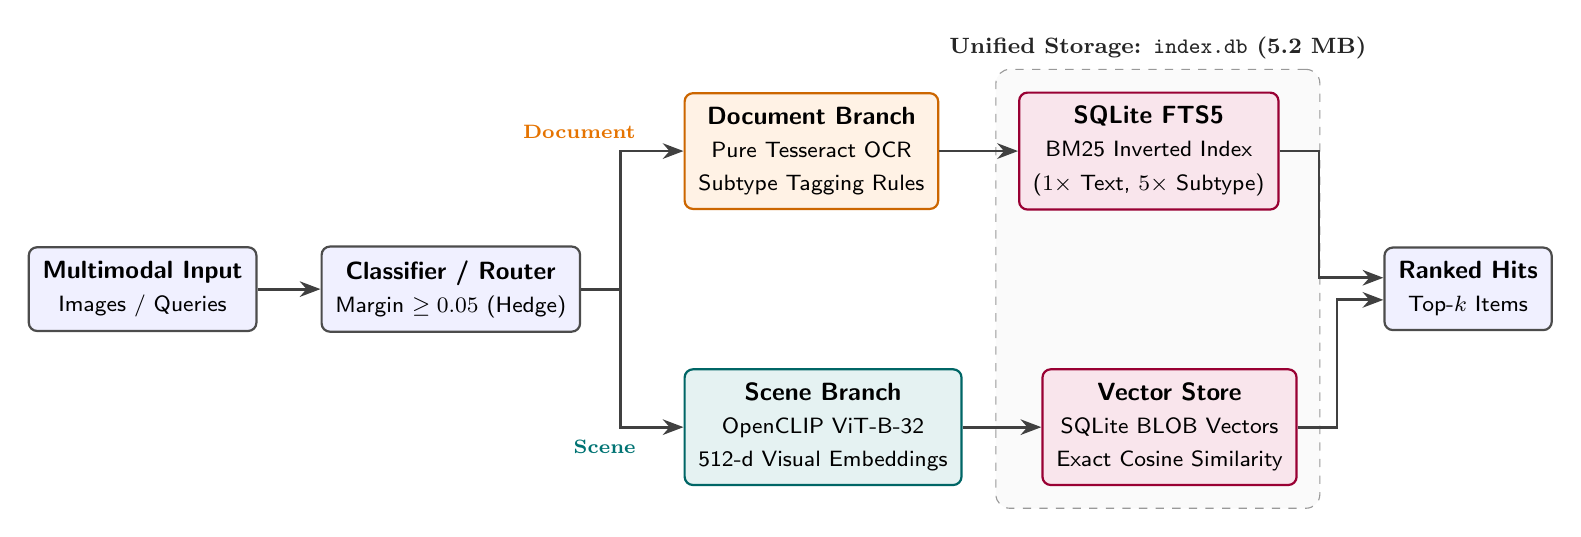
\begin{tikzpicture}[
    font=\sffamily\small,
    >=Stealth,
    thick,
    node distance=0.6cm and 0.9cm,
    block/.style={draw=black!70, rounded corners=3pt, fill=blue!6, align=center, inner sep=5pt, line width=0.8pt},
    docblock/.style={draw=orange!80!black, rounded corners=3pt, fill=orange!10, align=center, inner sep=5pt, line width=0.8pt},
    scnblock/.style={draw=teal!80!black, rounded corners=3pt, fill=teal!10, align=center, inner sep=5pt, line width=0.8pt},
    dbblock/.style={draw=purple!80!black, rounded corners=3pt, fill=purple!10, align=center, inner sep=5pt, line width=0.8pt},
    groupbox/.style={draw=black!40, dashed, rounded corners=5pt, fill=black!2, inner sep=8pt},
    arrow/.style={->, line width=1pt, draw=black!75}
]

% Inputs
\node[block] (input) {\textbf{Multimodal Input}\\[1pt]\footnotesize Images / Queries};

% Router / Classifier
\node[block, right=0.8cm of input] (router) {\textbf{Classifier / Router}\\[1pt]\footnotesize Margin $\ge 0.05$ (Hedge)};

% Document Branch (Top)
\node[docblock, above right=0.45cm and 1.3cm of router] (ocr) {\textbf{Document Branch}\\[1pt]\footnotesize Pure Tesseract OCR\\[1pt]\footnotesize Subtype Tagging Rules};

% Scene Branch (Bottom)
\node[scnblock, below right=0.45cm and 1.3cm of router] (clip) {\textbf{Scene Branch}\\[1pt]\footnotesize OpenCLIP ViT-B-32\\[1pt]\footnotesize 512-d Visual Embeddings};

% Unified Storage (index.db)
\node[dbblock, right=1.0cm of ocr] (fts) {\textbf{SQLite FTS5}\\[1pt]\footnotesize BM25 Inverted Index\\[1pt]\footnotesize ($1\times$ Text, $5\times$ Subtype)};

\node[dbblock, right=1.0cm of clip] (vec) {\textbf{Vector Store}\\[1pt]\footnotesize SQLite BLOB Vectors\\[1pt]\footnotesize Exact Cosine Similarity};

% Unified DB Container background
\begin{scope}[on background layer]
  \node[groupbox, fit=(fts) (vec), label={[font=\footnotesize\bfseries, text=black!85]above:Unified Storage: \texttt{index.db} (5.2 MB)}] (dbbox) {};
\end{scope}

% Output clearly to the right of the dbbox container
\node[block, right=0.8cm of dbbox.east] (output) {\textbf{Ranked Hits}\\[1pt]\footnotesize Top-$k$ Items};

% Arrows
\draw[arrow] (input) -- (router);

% Route fork with labels clearly placed above/below the horizontal branch
\draw[arrow] (router.east) -- ++(0.5,0) |- (ocr.west) node[pos=0.72, above left=1pt, font=\scriptsize\bfseries, text=orange!90!black] {Document};
\draw[arrow] (router.east) -- ++(0.5,0) |- (clip.west) node[pos=0.72, below left=1pt, font=\scriptsize\bfseries, text=teal!90!black] {Scene};

\draw[arrow] (ocr) -- (fts);
\draw[arrow] (clip) -- (vec);

% Arrows from FTS / Vector Store into Output
\draw[arrow] (fts.east) -- ++(0.5,0) |- ([yshift=4pt]output.west);
\draw[arrow] (vec.east) -- ++(0.5,0) |- ([yshift=-4pt]output.west);

\end{tikzpicture}%
}
\caption{Pixarch Dual-Branch Baseline Architecture.}
\label{fig:arch}
\end{figure}

\end{document}
